\section{Applications}
\label{sec:apps}

\subsection{Which decays are classical polarimeters}

\begin{table}[t]
\caption{Analysing powers of spin-$1/2$ decays when only the listed direction is recorded. A polarimeter is classical (noncontextual on all spin states) if and only if $|\kappa|\le1/3$. Leading order, $m_b=0$ and narrow $W$ for the top quark, with $m_t=\mtop\pm\mtopErr$ GeV and $m_W=\mW$ GeV \cite{pdg2026}; $x_0$ is a threshold on the scaled electron energy, Eq.~\eqref{eq:kappacut}.}
\label{tab:kappa}
\begin{ruledtabular}
\begin{tabular}{llc}
Decay & Recorded direction & $|\kappa|$\\
\hline
$t\to b\,\ell^+\nu$, $t\to b\,\bar d u$ & $\ell^+$ or $\bar d$ & $1$\\
 & $b$ (or $W$) & $\kappab$\\
 & $\nu$ or $u$ & $\kappanu\pm\kappanuErr$\\
$\mu\to e\nu\bar\nu$, $\tau\to\ell\nu\bar\nu$ & $e$, $\ell$ (all energies) & $1/3$\\
 & $e$ with $x>x_0>0$ & $>1/3$\\
$\tau\to\pi\nu$ & $\pi$ & $1$\\
$\tau\to\rho\nu$ & $\rho$ & $\taurho$\\
$\Lambda\to p\pi^-$ & $p$ & $0.752$\\
\end{tabular}
\end{ruledtabular}
\end{table}

Table~\ref{tab:kappa} collects analysing powers. Three entries sit at or near the boundary of Theorem~\ref{thm:half}.

\emph{Muon decay.} The direction-only electron asymmetry of the $V\!-\!A$ interaction has $|\kappa|=1/3$ exactly. The four-state model \eqref{eq:tetra} therefore reproduces the distribution $\frac{1}{4\pi}(1\mp\frac13\cos\theta)$ of fully polarised muons for every direction of the polarisation, and no polarimeter with a noncontextual model has a larger analysing power. Any threshold on the electron energy raises $|\kappa|$ above $1/3$, and the energy-resolved decay contains rank-one effects at the end point of the spectrum, so that recording the energy makes the fragment contextual for every $P>1/3$.

\emph{Top quark, $b$-quark direction.} From Eq.~\eqref{eq:kappab}, $|\kappa_b|>1/3$ if and only if $m_t>2m_W=\twomW$~GeV. At the measured masses $|\kappa_b|=\kappab$. The QCD correction computed in Ref.~\cite{brandenburg2002} lowers $|\kappa_b|$ by about $4\%$ at parton level, which does not change the conclusion: the $b$-quark (or $W$) direction is a nonclassical polarimeter.

\emph{Top quark, neutrino or up-type-quark direction.} Equation~\eqref{eq:kappanu} gives $|\kappa_\nu|=\kappanu\pm\kappanuErr$, the uncertainty being that of $m_t$; $|\kappa_\nu|=1/3$ at $\xi=\xistar$, that is, at $m_t=\mtstar$~GeV, $\mtstarPull$ standard deviations above the measured mass (Fig.~\ref{fig:half}b). In Ref.~\cite{brandenburg2002} the $b$-quark mass and the $W$ width together change this analysing power by $1.8\%$ (comparison of Eq.~\eqref{eq:kappanu} with the leading-order value given there) and the QCD correction changes it by $1.4\%$ at parton level and by $2$--$3\%$ for jets; each exceeds the distance of $1\%$ to the boundary. On which side of the boundary this polarimeter lies is therefore not decided by the leading-order formula. The charged-lepton direction is sharp up to a QCD correction of relative size $0.015\,\alpha_s$ \cite{brandenburg2002}; polarimeters built from jets have intermediate analysing powers \cite{brandenburg2002,tweedie2014}.

\begin{figure*}[t]
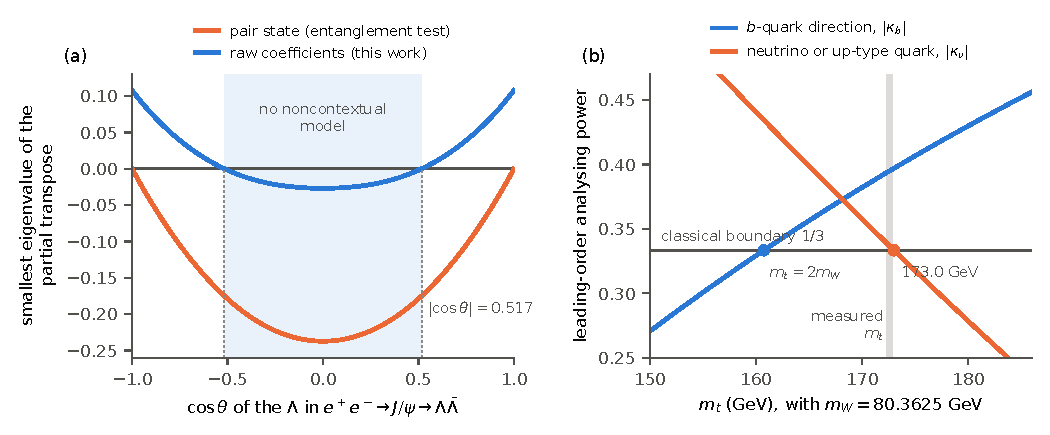
\includegraphics[width=0.86\textwidth]{fig_half}
\caption{(a) Smallest eigenvalue of the partial transpose for $e^+e^-\to J/\psi\to\Lambda\bar\Lambda$ with the BESIII parameters \cite{besiii2022}: of the pair state (the entanglement test) and of $\rhoraw$ built from the raw $p\bar p$ angular coefficients (Theorem~\ref{thm:pair}). The raw data have no noncontextual model in the shaded window. (b) Leading-order analysing powers of the $b$-quark and neutrino directions of top-quark decay against $m_t$; the band is the measured mass \cite{pdg2026}.}
\label{fig:half}
\end{figure*}

\subsection{Top-quark pairs}

ATLAS and CMS measure $D=-3\langle\cos\varphi\rangle$, with $\varphi$ the angle between the two charged-lepton directions, each in the rest frame of its parent top quark. ATLAS reports $D=\DATLAS\pm0.002\,(\text{stat})\pm0.019\,(\text{syst})$ at particle level for $340<m_{t\bar t}<380$~GeV, where the limit $-1/3$ corresponds to $\DATLASbound\pm0.009$ \cite{atlas2024}; CMS reports $D=\DCMS^{+0.026}_{-0.029}$ at parton level in its threshold region \cite{cms2024}. By Corollary~\ref{cor:D} noncontextual lepton-direction data satisfy $|D|\le1/3$, the same number as the separability limit for $|\kappa_\ell|=1$. The measurements therefore exclude a noncontextual model of the lepton-direction data at the significance obtained for entanglement: $\zCMS$ standard deviations for CMS, and $\zATLAS$ for ATLAS if the quoted uncertainties of the measurement and of the folded limit are added in quadrature (ATLAS states more than five).

Three points distinguish this reading from the entanglement reading of the same numbers. First, the bound $|D|\le1/3$ is derived for the raw coefficients and needs no value of the analysing power; the entanglement inference divides by $\kappa_\ell\bar\kappa_\ell$. Second, the statement concerns the data rather than the state: the local hidden-variable model that always exists for these data (Remark~\ref{rem:lhv}) is contextual, and every local model whose response functions are linear in the effects is excluded. Third, the two criteria separate for other decay channels. For unpolarised pairs $\|c\|_1=|\kappa_A\kappa_B|\,\|C\|_1\le3|\kappa_A\kappa_B|$. With the $b$-quark direction on both sides $\kappa_b^2=\kbsq$, so $\|c\|_1<1$ and the data are noncontextual for every spin state, entangled or not; with a neutrino or up-type-quark direction on one side the same holds if $|\kappa_\nu|\le1/3$ (Corollary~\ref{cor:weak}); with a charged lepton on one side and the $b$ quark on the other, contextuality requires $\|C\|_1>1/|\kappa_b|=\Cneed$. Only channels with the charged lepton or the down-type quark on both sides test contextuality at the level at which entanglement is tested.

The statements above are subject to the same qualifications as the entanglement measurements: the coefficient $D$ refers to the distribution unfolded to the full phase space, the limit at particle level is obtained from simulation, and the events of the selected region are averaged in an event-dependent basis. The last point does not affect Corollary~\ref{cor:D}: the trace of $c$ is basis independent, and the set of noncontextual coefficient matrices is convex.

\subsection{Hyperon pairs}

For $e^+e^-\to J/\psi\to\Lambda\bar\Lambda\to p\pi^-\bar p\pi^+$ the joint angular distribution is known in closed form \cite{faldt2017}. In the frame of Ref.~\cite{faldt2017}, with $\theta$ the production angle of the $\Lambda$ and $N=1+\alpha_\psi\cos^2\theta$, the pair state has polarisations $P_y=\sqrt{1-\alpha_\psi^2}\,\sin\Delta\Phi\,\sin\theta\cos\theta/N$ for both hyperons and correlations $C_{xx}=\sin^2\theta/N$, $C_{yy}=-\alpha_\psi\sin^2\theta/N$, $C_{zz}=(\alpha_\psi+\cos^2\theta)/N$, $C_{xz}=C_{zx}=\sqrt{1-\alpha_\psi^2}\,\cos\Delta\Phi\,\sin\theta\cos\theta/N$. The raw coefficients are $\ba=\alpha_-P_y\hat{\bm y}$, $\bb=\alpha_+P_y\hat{\bm y}$, $c=\alpha_-\alpha_+C$. With the BESIII values $\alpha_\psi=\alphapsi$, $\Delta\Phi=\dphi$, $\alpha_-=\alpham$, $\alpha_+=\alphap$ \cite{besiii2022}:

(i) At $\theta=90^\circ$ the pair is unpolarised and $\|c\|_1=|\alpha_-\alpha_+|(1+2\alpha_\psi)=\cnorm$ ($\cnormAvg\pm\cnormErr$ with the average decay parameter and uncorrelated uncertainties), above the bound of Corollary~\ref{cor:tstate}.

(ii) $\rhoraw$ fails the test of Theorem~\ref{thm:pair} for $|\cos\theta|<\cosc$ (between $\coscLo$ and $\coscHi$ when the parameters are shifted by their uncertainties), a window containing $\fracEvents\%$ of the events. Outside the window the $p\bar p$ angular data have a noncontextual model, although the $\Lambda\bar\Lambda$ state is entangled at every angle except $\cos\theta=\pm1$ (Fig.~\ref{fig:half}a). The reason is $|\alpha_-\alpha_+|=\alphaprod$: by Corollary~\ref{cor:ent} the decay data of an entangled state need not be contextual.

(iii) For $J/\psi\to\Sigma^+\bar\Sigma^-$ the decay parameters of $\Sigma^+\to p\pi^0$ are close to $\mp1$ \cite{besiii2020sigma}, the polarimeters are almost sharp, and the two tests nearly coincide; at $90^\circ$, $\|c\|_1=\cnormSigma\pm\cnormSigmaErr$.

These statements are conditional on the fitted form: they say that the distribution which BESIII has fitted has no noncontextual model in the window. A direct test would measure the fifteen raw moments $\langle q_{A,i}\rangle$, $\langle q_{B,k}\rangle$, $\langle q_{A,i}q_{B,k}\rangle$ in bins of $\cos\theta$, without the helicity-formalism parametrisation, and evaluate $\rhoraw$; Eq.~\eqref{eq:dipole} needs the nine correlation moments only. Bell-type tests with hyperon pairs \cite{tornqvist1981,besiii2025} use decay-angle data of the same kind under additional assumptions about the decay.

\subsection{Vector bosons and vector mesons}

\emph{One particle.} The lepton direction of $W\to\ell\nu$ has the kernel $(\eta_1,\eta_2)=(\pm1,1)$, that of $Z\to\ell^+\ell^-$ has $(A_\ell,1)$, a decay into two pseudoscalars has $(0,-2)$ and a decay into a massless lepton pair through a vector current $(0,1)$. All lie outside $\cR$ (Fig.~\ref{fig:regions}a). For the baryon direction in $J/\psi\to B\bar B$, parity conservation gives $\eta_1=0$ and the production-angle parameter $\alpha_\psi$ fixes $w_0=(1-\alpha_\psi)/(3+\alpha_\psi)$. By Corollary~\ref{cor:parity}, $J/\psi\to\Lambda\bar\Lambda$ ($w_0=\wzeroLambda<\tfrac15$) is a nonclassical polarimeter of the $J/\psi$ spin; $J/\psi\to\Sigma^+\bar\Sigma^-$, with $\alpha_\psi=\alphaSigma\pm\alphaSigmaErr$ \cite{besiii2020sigma}, has $w_0=\wzeroSigma\pm\wzeroSigmaErr$, $\zSigma$ standard deviations above the upper boundary $\tfrac35$; and $\psi(2S)\to\tau^+\tau^-$, with $x=m_\tau^2/M^2=\xtau\ge\tfrac18$ \cite{pdg2024}, is a classical polarimeter. These are statements about the measurement on all spin-$1$ states; in $e^+e^-$ annihilation only the mixture of helicities $\pm1$ along the beam is prepared.

\emph{Pairs.} Table~\ref{tab:pairs} gives the visibilities above which the decay data of an isotropic spin-$1$ pair are contextual. The values $5/8$ and $2/5$ are well above the entanglement threshold $1/4$, and pairs with a $Z\to\ell\ell$ decay give noncontextual data at every visibility, because $A_\ell$ is small. Vector-boson pairs from Higgs-boson decays or from diboson production are not in the isotropic family in general; for them Theorem~\ref{thm:onepair} does not apply, but Eq.~\eqref{eq:dipole} does: for any state of two spin-$1$ particles, noncontextual data obey $|\langle\bq_A\!\cdot\!\bq_B\rangle|\le1/3$.
